
% Options for packages loaded elsewhere
\PassOptionsToPackage{unicode=true}{hyperref}
\PassOptionsToPackage{hyphens}{url}
%
\documentclass[12pt, a4paper]{article}
\usepackage{lmodern}
\usepackage{geometry}
\geometry{a4paper, left=25mm, right=25mm, 
                   top=25mm,  bottom=25mm}
\usepackage{url}
\usepackage[T1]{fontenc}
\usepackage{polyglossia}
\setmonofont{DejaVu Sans Mono}[Scale=MatchLowercase]
\usepackage[newfloat]{minted}
\usemintedstyle[julia]{arduino}
\setminted{frame=lines,framerule=1pt,numbers=left, breaklines}
\usepackage{latexsym,exscale,stmaryrd,amsmath,amssymb}
\usepackage[math-style=TeX]{unicode-math}
\setmathfont{latinmodern-math.otf}
\newenvironment{code}{\captionsetup{type=listing}}{}
\usepackage[font=small,labelfont=bf]{caption}
\SetupFloatingEnvironment{listing}{name=Code}
\usepackage{textcomp} % provides euro and other symbol
\usepackage{mathtools}
\bibliographystyle{siam}
\setlength{\parindent}{0pt}
\setlength{\parskip}{6pt plus 2pt minus 1pt}
\usepackage{xcolor}
\usepackage{hyperref}
\usepackage{color}
\usepackage{fancyvrb}
\usepackage{algpseudocode}
\usepackage{algorithm}
\usepackage{graphicx,grffile}
\usepackage{subcaption}
\usepackage{float}
\usepackage{courier}
\usepackage{tikz}
\usetikzlibrary{bayesnet}
\usepackage{ulem}
\usepackage{booktabs}
\usepackage{multirow}

\makeatletter
\renewcommand{\paragraph}{\@startsection{paragraph}{4}{0ex}%
    {-3.25ex plus -1ex minus -0.2ex}%
    {1.5ex plus 0.2ex}%
    {\normalfont\normalsize\bfseries}}
\makeatother
 
\stepcounter{secnumdepth}
\stepcounter{tocdepth}

\title{DPMM.jl}
\author{
  Ekin Akyürek\\
   CSAIL, Massachusetts Institute of Technology\\
   Koç University\\
  \texttt{akyurek@mit.edu}
 }



\begin{document}

\maketitle
\begin{abstract}
    
\end{abstract}
\newpage
\tableofcontents

\newpage


\section{Introduction}

This document is a  on a parallel implementation of Dirichlet process mixture
models (DPMM) in Julia by Ekin Akyürek with supervision of John
W. Fischer. In the following sections, we will explain DPMMs and present different samplers. Then, we will elucidate the software architecture of DPMM.jl\footnote{\url{https://github.com/ekinakyurek/DPMM.jl}} to demonstrate composability and expressiveness of the package. In the final section, we will compare the speed and convergence properties of the implemented samplers. Finally, we will benchmark our package with the existing DPMM softwares.

\section{Background}

\subsection{Mixture Models}

Mixture models are statistical models for representing data which comes from a set of different probability distributions. A mixture model is generally
parameterized through a mixture (i.e component) of parameters and weights assigned to each distribution which can be considerd as prior probabilities of the mixtures in the Bayesian
setting. The more weight attached to a mixture, the more data is generated from
that mixture. In this work, we will mostly use the notation presented in the document\cite{kamper2013gibbs}:

\subparagraph{Data}
\begin{center}
\begin{tabular}{|l|l|}
\hline
$N$ & Number of data vectors \\
$D$ & Dimension of data vectors \\
$x_i \in R^D$ & $i^th$ data vector \\
$X = (x_1, x_2,...,x_N)$ & Set of data vectors \\
$X_{\setminus i}$ & Set of data vectors, excluding $x_i$\\
$X_k$  & Set of data vectors from mixture component $k$ \\ 
$X_{k \setminus i}$  & Set of data vectors from mixture component $k$, excluding $x_i$\\
$N_k$ & Number of data vectors from mixture component $k$ \\  
$N_{k \setminus i}$ & Number of data vectors from mixture component $k$, except $x_i$\\ \hline
\end{tabular}
\end{center}

\subparagraph{Model}
\begin{center}
\begin{tabular}{|l|l|} \hline
$K$ & Number of components in a finite mixture model \\
$z_i$ & Discrete latent state indicating the component observation $x_i$ belongs to \\
$\mathbf{z} = (z_1, z_2,...,z_N)$ & Latent states for all observations $x_i,..., x_n$\\
$\mathbf{z}_{\setminus i}$ & Set of all latent states, excluding $z_i$\\
$\theta_k$  & Component parameters (e.g. $\mu_k$, $\Sigma_k$ in a Gaussian mixture model)  \\
$\pi_k$ & Prior probability that data vector $x_i$ will be assigned to mixture component $k$ \\
$\pi = (\pi_1,\pi_2,...,\pi_K)$ & Vector of prior assignment probabilities for each of $K$ components \\
$\beta$ & Hyper-parameters of the prior for $\theta$ in a Bayesian setting \\ \hline
\end{tabular}
\end{center}


\subsection{Dirichlet Process Mixture Models (DPMM)}

\subsubsection{Dirichlet Process (DP)}

There are many ways to interpret DP which are discussed in the following sections in detail. Formally, it is a random process
whose realizations are probability distributions. Moreover, the constructive
definition of Dirichlet process relies on the stick-breaking processes. Also,
Chinese Restaurant Process(CRP) and Pólya Urn Scheme also lead to DP.
All these definitions are related with each other according to
\href{https://en.wikipedia.org/wiki/De_Finetti\%27s_theorem}{de
Finetti's exchangeability theorem}.

DP is parameterized by concentration parameter \(\alpha\) and \(G_0\)
base distribution. One can show that \(\alpha\) controls how similar
draws will be to the \(G_0\). G is used to denote samples drawn from
DP.


\paragraph{Stick-Breaking Construction}

Stick-Breaking provides a simple way to draw samples from DP, but it requires countably infinite summation to be performed. Stick-Breaking steps are
as follows.

\begin{align}
v_1,v_2,...,v_i,... & \sim Beta(1,\alpha) \\
\pi_i &= v_i \prod_{j=1}^{i-1}(1-v_j) \\ 
\theta_1,\theta_2,...,\theta_i,... & \sim G_0 \\
G & = \sum_{i=1}^{\infty}\pi_i\delta_{\theta_i}
\end{align}

Here \(\delta_{\theta_i}\) is an indicator function centered on
\(\theta_i\), namely \(\delta_{\theta_i}(\theta)\) is zero everywhere
except \(\theta=\theta_i\). Note that \(\pi_i\)'s approach to zero
as i goes to infinity which makes it possible to approximate G using a finite
summation instead of an infinite one.


\paragraph{Chinese Restaurant Process (CRP)}

Chinese restaurant process is a discrete process which is named after the
analogy of seating customers at tables in a restaurant. There is two options for every arriving customer, she can be seated in an existing table with others already seating at it or she can be assigned to an empty table. Let's say
there are customers \(1:N\) and we will seat each customer sequentially with the
following probabilities in Equation \ref{eq:probs}, where \(c_k\) is the number of customers currently seated at \(k^{th}\) table, \(i\) is current number of customers seated at all tables in the restaurant and $z_i$ is the label of the table that $i'th$ customer is seated.
\begin{equation}
z_i|z_1,...,z_{i-1} = \begin{cases}
P(z_i=k)=\frac{c_k}{i-1+\alpha} & \text{for an existing table} \\
P(z_i=K+1)=\frac{\alpha}{i-1+\alpha} & \text{for opening a new table}
\end{cases}
\end{equation}\label{eq:probs}

Note that this processes is independent of the arriving order of customers. This is called the exhangeability property of CRP \cite{fang2016dirichlet}.

If we assume a base measure \(G_0\) as a prior for table/cluster
parameters and assign each table a probability measure sampled from
\(G_0\), the process becomes CRP Mixture Model or Pólya Urn Scheme.

\begin{align}
\theta_1...,\theta_K,... &\sim G_0 \\
z_i|z_1,...,z_{i-1} &= \begin{cases}
P(z_i=k)=\frac{c_k}{i-1+\alpha} & \text{for an existing table/cluster} \\
P(z_i=K+1)=\frac{\alpha}{i-1+\alpha} & \text{for opening a new table/cluster}
\end{cases}\\
X_i|z_i &\sim f(X_i|\theta_{z_i})
\end{align}

Exchangeability allows us to show that above model is equivalent to \cite{blackwell1973ferguson}:

\begin{align*}
G &\sim DP(\alpha,G_0)  \\
\theta_i|G &\sim G \qquad i \in 1,...,N \\
X_i|\theta_i &\sim  f(X_i|\theta_i) \qquad i \in 1,...,N \\
\end{align*}

\paragraph{Formal Definition}

We stated that samples from a Dirichlet process are probability
distribution themselves. Let one these samples to be a probability distribution over the space $S$. Let \(\{A_i\}_{i=1}^n\) denote a measurable partition of S. For
any measurable partition of S below statement holds (\(Dir\) is
Dirichlet Distribution):

\begin{equation*}
G \sim DP(\alpha,G_0) \implies  (G(A_1),G(A_2),...,G(A_N)) \sim Dir(\alpha G_0(A_1),...,\alpha G_0(A_N))
\end{equation*}

This defines a Dirichlet Process, however it doesn't allow to draw samples relying on this definition unlike CRP or Pólya Urn.


\subsubsection{Infinite Mixture Models}

As we show in CRP section, Dirichlet process is a very good prior on
mixture models' parameters as it can model infinite number of clusters.
Note that every finite data realization of DPMM is a finite mixture
model with Dirichlet distribution as shown in the formal definition. One can
use finite a stick-breaking process to construct a DP, however it results in
approximation errors. On the other hand, CRP Mixture Model provides an
exact way of sampling and enables inference on the mixture data. Finally,
these two different representations are summarized in Figure \ref{pgm}. The following section discusses how to
do inference on DPMM.


\begin{figure}[ht]
  \begin{center}
    \begin{tabular*}{0.7\textwidth}{c @{\extracolsep{\fill}} c}

\begin{tikzpicture}
  % Define nodes
  \node[obs] (xi) {$x_i$}; %
  \node[latent, above=of xi] (thetai) {$\theta_i$}; %
  \node[latent, above=of thetai] (G) {$G$};
  \node[det, left=of G] (alpha) {$\alpha$};
  \node[det, above=of G] (G0) {$G_0$};
  \edge[]{thetai}{xi};
  \edge[]{G}{thetai};
  \edge[]{alpha}{G};
  \edge[]{G0}{G};
  \plate{}{ %
    (thetai)
    (xi)
  } {$N$} ;
\end{tikzpicture}
&
\begin{tikzpicture}
  % Define nodes
  \node[obs] (xi) {$x_i$}; %
  \node[latent, above=of xi] (zi) {$z_i$}; %
  \node[latent, above=of zi] (pi) {$\pi$};
  \node[det, left=of pi] (alpha) {$\alpha$};
  \node[latent, right=of pi] (theta) {$\theta$};
  \node[det, above=of theta] (G0) {$G_0$};
  \edge[]{zi}{xi};
  \edge[]{pi}{zi};
  \edge[]{alpha}{pi};
  \edge[]{theta}{xi};
  \edge[]{G0}{theta};
  \plate{xizi}{ %
    (zi)
    (xi)
  } {$N$} ;
  \plate{g0theate}{
    (G0)
    (theta)
  }{$\infty$};
\end{tikzpicture}

    \end{tabular*}
  \end{center}
  \caption{Two equivalent graphical representation of DPMM}
\end{figure}

%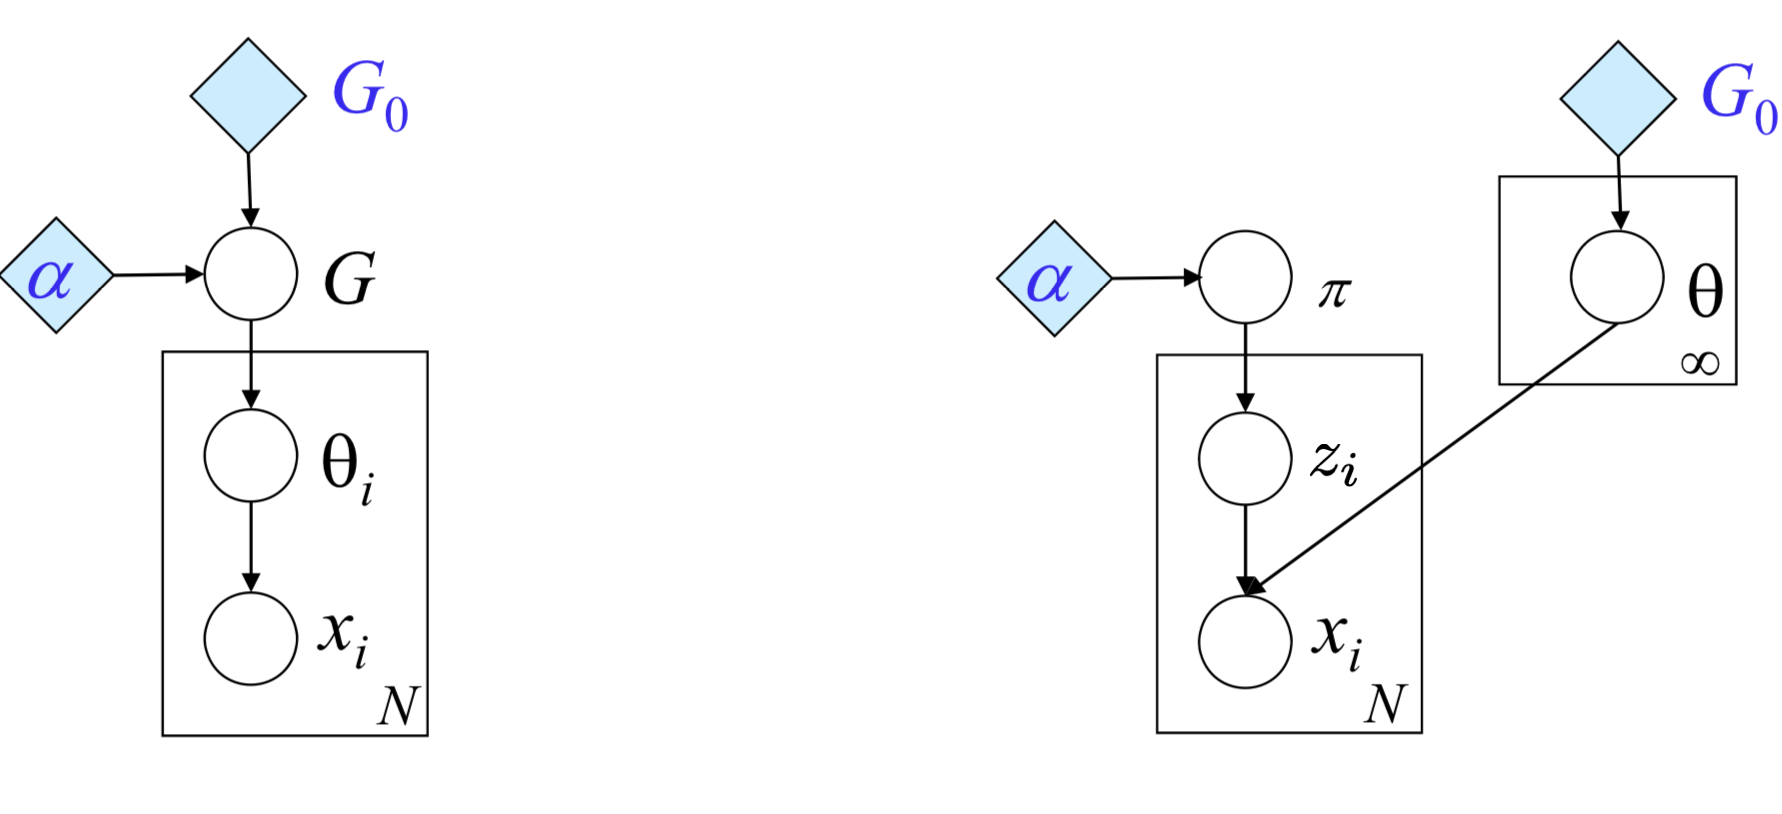
\includegraphics[width=\textwidth]{img/pgm-dpgmm.png}

\subsection{Inference in DPMM}

Inference problem that we interested in is to obtain cluster assignments
for each data point given base distribution \(G_0\) and \(\alpha\)
parameter. We will use conjugate prior which assures that the posterior
probability of cluster parameters are in the same distribution family with
the prior. Let's investigate conjugate priors for Gaussian and
Multinomial distributions.

\subsubsection{Posteriors \& Sufficent Statistics}

\paragraph{Gaussian Conjugate: Normal-Wishart Distribution}

Multivariate Gaussian Distribution is generally parameterized by a mean vector
\(\mu\) and covariance matrix \(\Sigma\). However, this parameterization results in expensive likelihood computations due to $\Sigma^{-1}$ term in the pdf function. Therefore, we prefer precision $J$ and $\mu$ parameterization. Normal-Wishart(NW)
Distribution\cite{murphy2007conjugate} is the prior distribution for Gaussian with unknown \(\mu\) and unknown $J$.

Normal-Wishart is parameterized by:

\begin{center}
\begin{tabular}{|l|l|}
\hline
 $\boldsymbol \mu_0$  & prior mean for $\mu$ \\ 
 $\boldsymbol \Psi_0$ & proportional to prior mean $\Sigma$\\
 $\lambda_0$ & how strongly we believe in $\mu_0$\\
 $\nu_0$ & how strongly we believe in $\Psi_0$\\ 
 \hline
\end{tabular}
\end{center}

NW has separable pdf function composed of a Gaussian and
a Wishart(\(\mathcal{W}\)) distribution.
\begin{equation*}
p(\boldsymbol\mu,\boldsymbol J|\boldsymbol\mu_0,\lambda_0,\boldsymbol\Psi_0,\nu_0) = \mathcal{N}\left(\boldsymbol\mu\Big|\boldsymbol\mu_0,\lambda\boldsymbol J\right) \mathcal{W}(\boldsymbol J|\boldsymbol\Psi_0,\nu_0)
\end{equation*}
To better understand how to sample from Wishart distribution
see the reference for the Bartlett decomposition method \cite{wishart1928generalised}. If we use sample mean(\(\hat{\mu}\)) and sample
covariance(\(\hat{\Sigma}\)) matrix as sufficient statistics, posterior
parameters for the Normal-Wishart distribution is given by the
below equations 9 to 13 \cite{kamper2013gibbs}:

%Instead of using Distributions.jl package, we had to define above distributions and sampling functions in the code due to performance reasons.



\begin{align}
p(\boldsymbol\mu,\boldsymbol J|\mathcal{X}) & = NW(\boldsymbol\mu,\boldsymbol J| \boldsymbol  \mu_N,  \boldsymbol  \Psi_N, \lambda_N, \nu_N)  \\
\boldsymbol \mu_N & = \lambda_0 \boldsymbol \mu_0 + N \hat{\mu} \\
\lambda_N & = \lambda_0 + N \\
\nu_N & = \nu_0 + N \\
\boldsymbol \Psi_N &=  \Psi_0 + \hat{\Sigma} + \frac{\lambda_0N}{\lambda_0+N}(\hat{\mu}-\boldsymbol \mu_0)(\hat{\mu}-\boldsymbol \mu_0)^T
\end{align}

It is also possible to store \(t =N\hat{x}\) and \(T=\sum_{i=1}^Nxx^T\)
as sufficient statistics, which is computationally more efficient. Then the
equations become:

\begin{align*}
\boldsymbol \mu_N & = \lambda_0 \boldsymbol \mu_0 + t \\
\lambda_N & = \lambda_0 + N \\
\nu_N & = \nu_0 + N \\
\boldsymbol \Psi_N &=  \Psi_0 + T + \lambda_0\boldsymbol\mu_0\boldsymbol\mu_0^T-\lambda_N\boldsymbol\mu_N\boldsymbol\mu_N ^T
\end{align*}


\subparagraph{Low-Rank Updates for
\(\Psi_N\)}

In the code, we store \(\Psi_N\) in Cholesky factorized form to sample from it
efficiently. However, we need to calculate Cholesky factorization, which is an
$\mathcal{O}(n^3)$ operation, every time if we remove or add single data point.
To overcome this challenge, there is a fast algorithm to compute the updated Cholesky
factorization from the previous Cholesky factorization \cite{Seeger:161468}. We utilize Rank-1
update and Rank-1 down-date methods to speed up the collapsed Gibbs sampler.


\paragraph{Multinomial Conjugate: Dirichlet Distribution}

Multinomial probability distribution is used for mixture distribution for discrete data, and Dirichlet distribution is the conjugate prior for Multinomial distribution. Dirichlet distribution is parameterized by $\vec{\alpha}$ where $\vec{\alpha}_i$ corresponds to pseudo-count of Multinomial event $i$. In addition to, we also store the logarithm of $\vec\alpha$ values for fast log-likelihood computations. The likelihood of probabilities of a Multinomial distribution given by a Dirichlet prior is:

\begin{equation}
f(p_{1},\ldots ,p_{K};\vec{\alpha}_{1},\ldots ,\vec{\alpha}_{K})=\frac {1}{\mathrm {B} ({\boldsymbol {\alpha }})} \prod _{i=1}^{K}p_{i}^{\vec{\alpha_{i}}-1}
\end{equation}

Sufficient statistics $t$ for Dirichlet prior and Multinomial distribution is the count vector of events $t=\vec{c}$ where:

$$\vec{c}_i = \sum_{j=1}^N{\mathcal{X}_{ik}}$$

Then, posterior distribution of Dirichlet is given by:

$$\vec{\alpha}^\prime  = \vec{\alpha}+ \vec{c}$$

\paragraph{Notes on Non-Conjugate Distributions}

Posteriors to non-conjugate priors should be calculated as a multiplication of prior and data likelihood. In this case, it does not create an analytic distribution, thus, cannot be normalized analytically. Hence, one should program an effective sampler for this type of posteriors. 



\subsubsection{Collapsed Gibbs Sampler}

When using conjugate priors for cluster parameters, marginal likelihood
of data can be obtained by analytically integrating out the cluster
parameter, \(\theta_i\). For Gaussian parameters the marginal
likelihood is

\begin{equation*}
p(\mathcal{X}) = \int_\mu\int_\Sigma p(\mathcal{X},\mu,\Sigma)p(\mu,\Sigma)d\mu d\Sigma
\end{equation*}

The likelihood of a new data \(x^*\) is given by
\begin{equation*}
p(x^* | \mathcal{X}) = \frac{p(x^*,\mathcal{X})}{p(\mathcal{X})}
\end{equation*}

It turns out that the posterior likelihood (posterior-predictive) of new data has Multivariate Student's t-distribution \cite{kamper2013gibbs} for NW-Gaussian pair:
\begin{equation*}
    p(x^*|\mathcal{X}) = \mathcal{T}(x^*|\boldsymbol \mu_N,\frac{(\lambda_N+1)}{\lambda_N(\nu_N-D+1)} \boldsymbol\Psi_N,\nu_n-D+1)
\end{equation*}

The posterior predictive likelihood of Dirichlet-Multinomial pair has a rather complicated definition:
\begin{equation*}
     p(x^*|\mathcal{X}) = \frac{\Gamma(n+1)}{\prod_{j=1}^{K}\Gamma(x^*_j+1)} \frac{\Gamma(\sum_{j=1}^{K}\alpha^\prime_j)}{\prod_{j=1}^{K}\Gamma(\alpha^\prime_j)} 
     \frac{\prod_{j=1}^{K}\Gamma(x^*_j+\alpha^\prime_j)}{\Gamma(n+\sum_{j=1}^{K}\alpha^\prime_j)}
\end{equation*}

The collapsed inference in DPMM can be done by using CRP
procedure. The difference is that instead of using \(f(x|\theta_{z_i})\)
likelihood, we use  $p(x^*|\mathcal{X})$ 
posterior-predictive and we never sample \(\theta\)'s
explicitly \cite{kamper2013gibbs}.

\begin{align*}
z_i|\boldsymbol z_{\setminus i}  &\sim \begin{cases}
P(z_i=k)=p(x|\beta,\mathcal{X}_{k \setminus i})\frac{N_{k\setminus i}}{N-1+\alpha} & \text{for an existing table/cluster} \\
P(z_i=K+1)=p(x|\beta)\frac{\alpha}{N-1+\alpha} & \text{for a new table/cluster}
\end{cases}
\end{align*}

Pseudo-code \cite{kamper2013gibbs} of collapsed gibbs sampler is presented in Algorithm \ref{collapsedgibbs}.


\begin{algorithm}
  \caption{Collapsed Gibbs sampler for an infinite mixture model.}\label{collapsedgibbs}
  \begin{algorithmic}[1]
    
  \State Choose an initial \textbf{z}.
  \For{M iterations} \Comment{Gibbs Sampling Iterations}
    \For{i = 1 to N}
        \State Remove $\mathbf{x}_i's$ statistics from component $z_i$ \Comment{Old assignment for $\mathbf{x}_i$}
        \For{k = 1 to K} \Comment{For all existing clusters}
            \State Calculate $P(z_i = k | \mathbf{z}_{\setminus i},\alpha) = \frac{N_{k\setminus i}}{N+\alpha-1}$ as in CRP
            \State Calculate $p(\mathbf{x}_i|\mathcal{X}_{k\setminus i},\mathbf{\beta})$ using posterior predictive distribution.
            \State Calculate $P(z_i = k | \mathbf{z}_{\setminus i},\mathcal{X},\alpha,\mathbf{\beta}) \propto P(z_i = k | \mathbf{z}_{\setminus i},\alpha) p(\mathbf{x}_i|\mathcal{X}_{k\setminus i}, \mathbf{\beta})$
        \EndFor
        \State Calculate $P(z_i = K+1 | \mathbf{z}_{\setminus i},\alpha) = \frac{\alpha}{N+\alpha-1}$ as in CRP \Comment{Consider opening a new cluster}
        \State Calculate $p(\mathbf{x}_i|\mathbf{\beta})$ using prior-predictive distribution.
        \State Calculate $P(z_i = K+1 | \mathbf{z}_{\setminus i},\mathcal{X},\alpha, \mathbf{\beta}) \propto P(z_i = K+1 | \mathbf{z}_{\setminus i},\alpha)p(\mathbf{x}_i|\mathbf{\beta})$
        \State Sample $k_{new}$ from $P(z_i = k | \mathbf{z}_{\setminus i},\mathcal{X},\mathbf{\alpha},\mathbf{\beta})$ after normalizing
        \State Add $z_i$'s statistics to the component $z_i = k_{new}$.\Comment{New assignment for $\mathbf{x}_i$}
        \State If any component is empty, remove it and decrease K
    \EndFor
  \EndFor
  \end{algorithmic}
\end{algorithm}


\subparagraph{Remarks}
\begin{enumerate}
   \item  \textbf{Parallelism Over Data Points:} Collapsed sampler cannot be parallelized over data points, because for each data point we need to update the cluster statistics, yet we don't know which cluster's statistic will change and what they will be beforehand.
   \item  \textbf{Parallelism Over Clusters:} Collapsed sampler \textit{can} be parallelized over clusters on the calculation of data likelihoods. Typically, $K$ is significantly less than $N$, so cluster parallelism does not help much.
   \item  \textbf{Empirical Convergence}:
  Collapsed sampler converges slowly when it starts with an underestimated
  number of clusters in which case close clusters tend to form a single cluster.
\end{enumerate}

\subsubsection{Quasi-Collapsed Gibbs Sampler}

Note that in collapsed sampling every latent variable $z_i$ is connected with each other in the undirected representation of DP.

\begin{center}
\begin{tikzpicture}
  \node[obs] (z1) {$z_1$}; %
  \node[obs, right=of z1] (z2) {$z_2$}; %
  \node[obs, right=of z2] (empty) {...};
  \node[obs, right=of empty] (zn) {$z_n$}; %
  \draw[-, >=latex, draw=black, black, thick, controls=+(90:2) and +(90:2)] (z1.north) to (zn.north);
  \draw[-, >=latex, draw=black, black, thick, controls=+(90:1) and +(90:1)] (z1.north) to (z2.north);
  \draw[-, >=latex, draw=black, black, thick, controls=+(90:1) and +(90:1)] (z2.north) to (zn.north);
  \draw[-, >=latex, draw=black, black, thick, controls=+(270:1) and +(270:1)] (empty.south) to (zn.south);
   \draw[-, >=latex, draw=black, black, thick, controls=+(270:1) and +(270:1)] (empty.south) to (z2.south);
\draw[-, >=latex, draw=black, black, thick, controls=+(270:1.5) and +(270:1.5)] (empty.south) to (z1.south);
\end{tikzpicture}
\end{center}

So, it is not possible to sample $z_i$'s in parallel for an exact sampling. However, the affect of change in $z_i$ is negligible when $N \rightarrow \infty$. Therefore, we can break above connections for an approximate collapsed sampling algorithm which is parallelizable. It also corresponds to removing $4^{th}$ and $14^{th}$ lines, and calculation of posterior-predictive distribution before the iteration in Algorithm \ref{collapsedgibbs}. So, in this revised version of the algorithm, instead of updating posterior-predictive for each data point, we update it only in the beginning of an iteration. The quasi-collapsed sampler algorithm is presented in Algorithm \ref{quasicollapsedgibbs} and sampling scheme is presented in the equation:

\begin{align*}
z_i|\boldsymbol z &\sim \begin{cases}
P(z_i=k)=p(x|\beta,\mathcal{X}_{k})\frac{N_{k}}{N+\alpha} & \text{for an existing table/cluster} \\
P(z_i=K+1)=p(x|\beta)\frac{\alpha}{N+\alpha} & \text{for a new table/cluster}
\end{cases}
\end{align*}

\subparagraph{Remarks}
\begin{enumerate}
   \item  \textbf{Parallelism Over Data Points:} Quasi-Collapsed sampler can be parallelized over data points, since we do not update cluster statistics during an iteration.
   \item  \textbf{Parallelism Over Clusters:} Quasi-Collapsed sampler can be parallelized over clusters for the calculation of data likelihoods. Calculation of posterior-predictive distributions is also parallelizable. In most practical examples, $K$ is significantly less than $N$, so cluster parallelism does not help much.
   \item  \textbf{Empirical Convergence}: Quasi-Collapsed sampler sometimes does not converge to correct number of clusters. Closer clusters tend to form a single cluster in that situation.
\end{enumerate}

\begin{algorithm}[H]
  \caption{Quasi-Collapsed Gibbs sampler for an infinite mixture model.}\label{quasicollapsedgibbs}
  \begin{algorithmic}[1]
  \State Choose an initial \textbf{z}.
  \For{M iterations} \Comment{Gibbs Sampling Iterations}
    \State \textcolor{blue}{Update posterior-predictive distributions with \textbf{z}}
    \For{i = 1 to N}
        %\State \sout{Remove $\mathbf{x}_i's$ statistics from component $z_i$} \Comment{Old assignment for $\mathbf{x}_i$}
        \For{k = 1 to K} \Comment{For all existing clusters}
            \State Calculate $P(z_i = k | \mathbf{z},\alpha) = \frac{N_{k}}{N+\alpha}$ as in CRP
            \State Calculate $p(\mathbf{x}_i|\mathcal{X}_{k},\mathbf{\beta})$ using posterior predictive distribution \textcolor{blue}{with old assignments \textbf{z}}
            \State Calculate $P(z_i = k | \mathbf{z},\mathcal{X},\alpha,\mathbf{\beta}) \propto P(z_i = k | \mathbf{z},\alpha) p(\mathbf{x}_i|\mathcal{X}_{k}, \mathbf{\beta})$
        \EndFor
        \State Calculate $P(z_i = K+1 | \mathbf{z},\alpha) = \frac{\alpha}{N+\alpha}$ as in CRP \Comment{Consider opening a new cluster}
        \State Calculate $p(\mathbf{x}_i|\mathbf{\beta})$ using prior-preditive distribution.
        \State Calculate $P(z_i = K+1 | \mathbf{z},\mathcal{X},\alpha, \mathbf{\beta}) \propto P(z_i = K+1 | \mathbf{z},\alpha)p(\mathbf{x}_i|\mathbf{\beta})$
        \State Sample $k_{new}$ from $P(z_i = k | \mathbf{z},\mathcal{X},\mathbf{\alpha},\mathbf{\beta})$ after normalizing
        %\State \sout{ Add $z_i$'s statistics to the component $z_i = k_{new}$.}\Comment{New assignment for $\mathbf{x}_i$}
    \EndFor
    \State If any component is empty, remove it and decrease K

  \EndFor
  \end{algorithmic}
\end{algorithm}

\subsubsection{Direct Gibbs Sampler}

Collapsed and Quasi-Collapsed algorithms use CRP procedure to construct DP. However, there is another approach from which mixture weights and mixture parameters are sampled directly. There is, however, an infinite number of clusters in DP, but we can represent uninstantiated clusters' weights by a single probability $\pi_{K+1}$. So, $\pi_{K+1}$ is the sum of all uninstantiated cluster weights and $\theta_{K+1}$ is sampled from the base distribution for a new cluster. Direct sampler scheme is given in the below:

\begin{align*}
\pi_1...,\pi_K, \pi_{K+1} &\sim Dir\big(N_1,...,N_K, \alpha \big) \\
\theta_1...,\theta_K&\sim G_0(\theta|\boldsymbol z, \beta) \\
z_i|\boldsymbol z &\sim \begin{cases}
P(z_i=k)= f(X_i|\theta_{k})\pi_k & \text{for an existing cluster} \\
P(z_i=K+1)= f(X_i|\theta_{K+1})\pi_{K+1}& \text{for a new cluster}
\end{cases}\\
\end{align*}

\begin{enumerate}
   \item  \textbf{Parallelism Over Data Points:} Direct sampler can be parallelized over data points.
   \item  \textbf{Parallelism Over Clusters:} Direct sampler can be parallelized over clusters for likelihood calculations. Sampling of $\theta$ parameters is also parallelizable in a similar fashion. In practice, $K$ is significantly less than $N$, so cluster parallelism does not help much.
   \item  \textbf{Empirical Convergence}:
  Direct sampler converges slowly when it instantiated with underestimated
  number of clusters in which case closer clusters tend to form a single cluster.
\end{enumerate}

\begin{algorithm}[H]
  \caption{Direct Gibbs sampler for an infinite mixture model.}\label{directgibbs}
  \begin{algorithmic}[1]
    
  \State Choose an initial \textbf{z}.
  \For{M iterations} \Comment{Gibbs Sampling Iterations}
    \For{k = 1 to K} \Comment{For all existing clusters}
            \State Sample $\theta_k \sim G_0(\theta|\beta,\mathcal{X}_{k})$ \Comment{if $N_k \neq 0$}
    \EndFor
    \State Sample $(\pi_{1}, \pi_{2},...,\pi_{K+1}) \sim  Dir\big(N_1,...,N_K, \alpha \big)$
    \For{i = 1 to N}
        \For{k = 1 to K} \Comment{For all existing clusters}
            \State Calculate $p(\mathbf{x}_i|\mathbf{\theta}_k)$ using mixture distribution
            \State Calculate $P(z_i = k | \mathbf{z},\mathcal{X},\alpha,\mathbf{\beta}) \propto  \pi_k p(\mathbf{x}_i|\mathbf{\theta}_k)$
        \EndFor
        \State Calculate $p(\mathbf{x}_i|\theta_{K+1})$ using mixture distribution
        \State Calculate $P(z_i = K+1 | \mathbf{z},\mathcal{X},\alpha, \mathbf{\beta}) \propto  \pi_{K+1}p(\mathbf{x}_i|\mathbf{\theta}_{K+1})$
        \State $z_i \gets k_{new}$ from $P(z_i = k | \mathbf{z},\mathcal{X},\mathbf{\alpha},\mathbf{\beta})$ after normalizing
    \EndFor
  \EndFor
  \end{algorithmic}
\end{algorithm}


\subsubsection{Quasi-Direct Gibbs Sampler}

When $N \rightarrow \infty$, we can estimate $(\pi_{1}, \pi_{2},...,\pi_{K+1})$ with their proportions:
$$\pi_k = \frac{N_k}{N+\alpha},\pi_{K+1} = \frac{\alpha}{N+\alpha} $$

So, we can get faster algorithm which skips sampling from Dirichlet process:

\begin{align*}
\theta_1...,\theta_K&\sim G_0(\theta|\boldsymbol z, \beta) \\
z_i|\boldsymbol z_{\setminus i} &\sim \begin{cases}
P(z_i=k)= f(X_i|\theta_{k})\frac{N_k}{N+\alpha} & \text{for an existing cluster} \\
P(z_i=K+1)= f(X_i|\theta)\frac{\alpha}{N+\alpha} & \text{for a new cluster}
\end{cases}\\
\end{align*}

We iteratively repeat the above steps. Pseudocode of quasi-direct Gibbs sampler is presented in Algorithm \ref{quasi-directgibbs}.



\begin{algorithm}[H]
  \caption{Quasi-Direct Gibbs sampler for an infinite  mixture model.}\label{quasi-directgibbs}
  \begin{algorithmic}[1]
    
  \State Choose an initial \textbf{z}.
  \For{M iterations} \Comment{Gibbs Sampling Iterations}
    \For{k = 1 to K} \Comment{For all existing clusters}
            \State Sample $\theta_k \sim G_0(\theta|\beta,\mathcal{X}_{k})$ \Comment{if $N_k \neq 0$}
    \EndFor
    \For{i = 1 to N}
        \For{k = 1 to K} \Comment{For all existing clusters}
            \State Calculate $P(z_i = k | \mathbf{z},\alpha) = \frac{N_{k}}{N+\alpha}$ as in CRP
            \State Calculate $p(\mathbf{x}_i|\mathbf{\theta}_k)$ using mixture distribution
            \State Calculate $P(z_i = k | \mathbf{z},\mathcal{X},\alpha,\mathbf{\beta}) \propto P(z_i = k | \mathbf{z},\alpha)p(\mathbf{x}_i|\mathbf{\theta}_k)$
        \EndFor
        \State Calculate $P(z_i = K+1 | \mathbf{z},\alpha) = \frac{\alpha}{N+\alpha}$ as in CRP \Comment{Consider opening a new cluster}
        \State Calculate $p(\mathbf{x}_i|\theta^*)$ using mixture distribution
        \State Calculate $P(z_i = K+1 | \mathbf{z},\mathcal{X},\alpha, \mathbf{\beta}) \propto P(z_i = K+1 | \mathbf{z},\alpha)p(\mathbf{x}_i|\mathbf{\theta}_{K+1})$
        \State $z_i \gets k_{new}$ from $P(z_i = k | \mathbf{z},\mathcal{X},\mathbf{\alpha},\mathbf{\beta})$ after normalizing
    \EndFor
  \EndFor
  \end{algorithmic}
\end{algorithm}

\subparagraph{Remarks}
\begin{enumerate}
   \item  \textbf{Parallelism Over Data Points:} Same as Direct Sampler.
   \item  \textbf{Parallelism Over Clusters:}  Same as Direct Sampler.
   \item  \textbf{Empirical Convergence}:
    It doesn't converge robustly.
\end{enumerate}

\subsubsection{Split-Merge Gibbs Sampler}
DP Split-Merge algorithm \cite{Chang2013dpmm} is a parallelizable Gibbs sampler for DPMM. It converges well, is easily parallelizable and able to work with non-conjugate priors. Algorithm starts with a non-ergodic restricted sampler assigning cluster labels to data points without creating a new cluster as in equations \ref{ds:one} to \ref{ds:three}. Then, another sampler assigns sub-cluster labels within the existing clusters, equations \ref{eq:one1} to \ref{eq:two2}. Split moves are proposed over subclusters, while merge moves are proposed over existing clusters. Through split-merge moves, algorithm becomes ergodic and has limiting guarantees. Restricted sampler is similar to Direct Sampler, except that it does not create new clusters:

\begin{align}
\pi_1...,\pi_K, \pi_{K+1} &\sim Dir\big(N_1,...,N_K, \alpha \big) \label{ds:one} \\ 
\theta_1...,\theta_K&\sim G_0(\theta|\boldsymbol z, \beta) \\
z_i|\boldsymbol z &\sim P(z_i=k) \propto f(X_i|\theta_{k})\pi_k \label{ds:three}
\end{align}\label{eq:directsamplernonergodic}

Another sampler assigns subcluster labels for existing clusters as shown in below:

\begin{align}
(\bar{\pi}_{kl}, \bar{\pi}_{kr}) &\sim \mathrm{Dir}(N_{kl}+\alpha/2, N_{kr}+\alpha/2) \label{eq:one1} \\
\bar{\theta}_{k\{l,r\}} &\sim G_0(\theta|\bar{\boldsymbol z}_{k\{l,r\}}, \beta)  \\
\bar{z}_{i} &\sim \sum_{j \in \{l,r\}} \pi_{z_{i}}f_x(x_i;\bar{\theta}_{z_{i}j})I[\bar{z}_{i} = j]\label{e1:two2}
\end{align}

Split and Merge moves are proposed via Metropolis-Hastings method. With a specific proposal distributions split move's hasting ratio $H_{\text {split}}$ is:
$$
H_{\text {split}} = \frac{\alpha}{\Gamma\left(N_{k}\right) f_{x}\left(x_{I_{k} ; \lambda}\right)} \Gamma\left(N_{k l}\right) f_{x}\left(x_{I_{k l}} ; \lambda\right) \Gamma\left(N_{k r}\right) f_{x}\left(x_{I_{k r}} ; \lambda\right)
$$

For newly created clusters one can keep track of marginal data likelihood, $\overline{\mathcal{L}}_{m}=f_{x}\left(x_{\{m, \ell\}} ; \overline{\theta}_{m, \ell}\right) \cdot f_{x}\left(x_{\{m, r\}} ; \overline{\theta}_{m, r}\right)$, and defer split moves when $\mathcal{L}_{m}$ oscillates enough. This will save us from computing new auxiliary subcluster variables in each iteration.

Similarly merge move's hasting ratio is:

$$
H_{\text {merge}}=0.01 \frac{\Gamma\left(N_{k 1}+N_{k 2}\right)}{\alpha \Gamma\left(N_{k 1}\right) \Gamma\left(N_{k 2}\right)} \frac{p(x | \hat{z})}{p(x | z)} \frac{\Gamma(\alpha)}{\Gamma\left(\alpha+N_{k 1}+N_{k 2}\right)} \frac{\Gamma\left(\alpha / 2+N_{k 1}\right) \Gamma\left(\alpha / 2+N_{k 2}\right)}{\Gamma(\alpha / 2) \Gamma(\alpha / 2)}
$$

\begin{enumerate}
   \item  \textbf{Parallelism Over Data Points:} Restricted sampler can be parallelized over data points. So, the assignments of clusters and subclusters can be done in parallel for a data point.
   \item  \textbf{Parallelism Over Clusters:} Direct sampler can be parallelized over clusters on the calculation of data likelihoods. Sampling of $\theta$ and $\bar{\theta}$ parameters is also parallelizable in a similar fashion. In addition,  split moves can be proposed in parallel. However, in most practical problems, $K$ is significantly less than $N$, so cluster parallelism does not help much.
   \item  \textbf{Emprical Convergence}:
    Split merge has the best convergence characteristics compared to other methods investigated in this report.
\end{enumerate}

\begin{algorithm}[H]
  \caption{Split-Merge Gibbs sampler for an infinite  mixture model.}\label{split-mergegibbs}
  \begin{algorithmic}[1]
    
  \State Choose an initial \textbf{z}.
  \State Choose initial subcluster assignments $\bar{z}$.
  \For{M iterations} \Comment{Gibbs Sampling Iterations}
    \For{k = 1 to K} \Comment{For all existing clusters}
            \State Sample $\theta_k \sim  G_0(\theta|\beta,\mathcal{X}_{k})$ 
            \State Sample $\theta_{kr} \sim  G_0(\theta|\beta,\mathcal{X}_{k,r})$
            \State Sample $\theta_{kl} \sim  G_0(\theta|\beta,\mathcal{X}_{k,l})$ 
            \State Assign splitability by tracking $\mathcal{L}_{m}$ history. 
    \EndFor
    
    \State Sample $ (\pi_{1}, \pi_{2},...,\pi_{K+1})  \sim Dir\big(N_1,...,N_K, \alpha \big) $
    \State Sample $(\bar{\pi}_{kl}, \bar{\pi}_{kr}) \sim \mathrm{Dir}(N_{kl}+\alpha/2, N_{kr}+\alpha/2)$
    
    \For{i = 1 to N} \Comment{Restricted Sampler}
        \For{k = 1 to K} 
            \State Calculate $p(\mathbf{x}_i|\mathbf{\theta}_k)$ using mixture distribution
            \State Calculate $P(z_i = k | \mathbf{z},\mathcal{X},\alpha,\mathbf{\beta}) \propto \pi_k p(\mathbf{x}_i|\mathbf{\theta}_k)$
        \EndFor
        \State $z_i \gets k_{new}$ from $P(z_i = k | \mathbf{z},\mathcal{X},\mathbf{\alpha},\mathbf{\beta})$ after normalizing
        \State $\bar{z}_i \gets j_{new}$ from $P(\bar{z}_i = j | \mathbf{z},\mathcal{X},\mathbf{\alpha},\mathbf{\beta}) = \sum_{j \in \{l,r\}} \pi_{z_{i}}f_x(x_i;\bar{\theta}_{z_{i}j})I[\bar{z}_{i} = j]$ 
         \For{k = 1 to K} \Comment{Split Moves}
             \If{k is Splitable}
                 \State Calculate Hastings ratio and accept split move with $p=min(1,H)$.
                 \State $H_{\text {split}}=\frac{\alpha}{\Gamma\left(N_{k}\right) f_{x}\left(x_{I_{k} ; \lambda}\right)} \Gamma\left(N_{k l}\right) f_{x}\left(x_{I_{k l}} ; \lambda\right) \Gamma\left(N_{k r}\right) f_{x}\left(x_{I_{k r}} ; \lambda\right)$
             \EndIf
        \EndFor
         \For{k = 1 to K} \Comment{Merge Moves}
             \State Calculate Hastings ratio and accept merge move with p=min(1,H).
             \State $H_{\text {merge}}=0.01 \frac{\Gamma\left(N_{k 1}+N_{k 2}\right)}{\alpha \Gamma\left(N_{k 1}\right) \Gamma\left(N_{k 2}\right)} \frac{p(x | \hat{z})}{p(x | z)} \frac{\Gamma(\alpha)}{\Gamma\left(\alpha+N_{k 1}+N_{k 2}\right)} \frac{\Gamma\left(\alpha / 2+N_{k 1}\right) \Gamma\left(\alpha / 2+N_{k 2}\right)}{\Gamma(\alpha / 2) \Gamma(\alpha / 2)}$
        \EndFor
    \EndFor
  \EndFor 
  \end{algorithmic}
\end{algorithm}

\subsection{Parallel Inference} \label{sec:parallelinf}
Different kinds of parallelism can be implemented for the Gibbs sampling algorithms. We will consider parallelism in two different categories: parallelism over data points, parallelism over clusters. 

% \begin{figure}[ht]
  \begin{center}
    \begin{tabular*}{1.5\textwidth}{ll}
\begin{tikzpicture}[
  node distance=2.5cm,
  squarednode/.style={rectangle, draw=black!60, fill=white, thick, minimum size=10mm},
  every edge/.style={  % Sets the properties for each transition
            draw,
           ->,>=stealth,     % Makes edges directed with bold arrowheads
           auto,
           semithick}
]
  \node[squarednode] (M) {Master};
  \node[squarednode] (M1) [below left=6cm and 4.5cm of M] {M1};
  \node[squarednode] (M2) [below=6cm of M, right=2cm of M1] {M2};
  \node[squarednode] (M3) [below=6cm of M, right=2cm of M2]  {M3};
  \node[squarednode] (M4) [below=6cm of M, right=2cm of M3]  {M4};
  
  \node[squarednode] (W11) [below left=6cm and 4.5cm of M1]    {W11};
  \node[squarednode] (W12) [below=6cm of M1, right=2cm of W11]  {W12};
  \node[squarednode] (W13) [below=6cm of M1, right=2cm of W12]  {W13};
  \node[squarednode] (W14) [below=6cm of M1, right=2cm of W13]  {W14};
  
  \node[squarednode]  (W21) [below left=6cm and 4.5cm of M2]    {W21};
  \node[squarednode]  (W22) [below=6cm of M2, right=2cm of W21]  {W22};
  \node[squarednode]  (W23) [below=6cm of M2, right=2cm of W22]  {W23};
  \node[squarednode]  (W24) [below=6cm of M2, right=2cm of W23]  {W24};
  
    
  \node[squarednode]  (W31) [below left=6cm and 4.5cm of M3]    {W31};
  \node[squarednode]  (W32) [below=6cm of M3, right=2cm of W31]  {W32};
  \node[squarednode]  (W33) [below=6cm of M3, right=2cm of W32]  {W33};
  \node[squarednode]  (W34) [below=6cm of M3, right=2cm of W33]  {W34};
  
  \node[squarednode]  (W41) [below left=6cm and 4.5cm of M4]    {W41};
  \node[squarednode]  (W42) [below=6cm of M4, right=2cm of W41]  {W42};
  \node[squarednode]  (W43) [below=6cm of M4, right=2cm of W42]  {W43};
  \node[squarednode]  (W44) [below=6cm of M4, right=2cm of W43]  {W44};
  
  
  
  \draw (M) edge  [bend left=-40] node[left=1mm] {params} (M1);
  \draw (M) edge  [bend left=-20] node[] {params} (M2);
  \draw (M) edge  [bend left=0] node[] {params} (M3);
  \draw (M) edge  [bend left=20] node[] {params} (M4);
  \draw (M1) edge [bend left=30] node[right=1mm] {$T_1$} (M);
  \draw (M2) edge [bend left=10] node[left=3mm] {$T_2$} (M);
  \draw (M3) edge [bend left=-10] node[left=3mm] {$T_3$} (M);
  \draw (M4) edge [bend left=-10] node[right=1mm] {$T_4$} (M);
  
  
  
    
  \draw (M1) edge  [bend left=-40] node[left=1mm] {params} (W11);
  \draw (M1) edge  [bend left=-20] node[] {params} (W12);
  \draw (M1) edge  [bend left=0] node[] {params} (W13);
  \draw (M1) edge  [bend left=20] node[] {params} (W14);
  \draw (W11) edge [bend left=30] node[right=1mm] {$T_1$} (M1);
  \draw (W12) edge [bend left=10] node[left=3mm] {$T_2$} (M1);
  \draw (W13) edge [bend left=-10] node[left=3mm] {$T_3$} (M1);
  \draw (W14) edge [bend left=-10] node[right=1mm] {$T_4$} (M1);
    
  \draw (M2) edge  [bend left=-40] node[left=1mm] {params} (W21);
  \draw (M2) edge  [bend left=-20] node[] {params} (W22);
  \draw (M2) edge  [bend left=0] node[] {params} (W22);
  \draw (M2) edge  [bend left=20] node[] {params} (W23);
  \draw (W21) edge [bend left=30] node[right=1mm] {$T_1$} (M2);
  \draw (W22) edge [bend left=10] node[left=3mm] {$T_2$} (M2);
  \draw (W23) edge [bend left=-10] node[left=3mm] {$T_3$} (M2);
  \draw (W24) edge [bend left=-10] node[right=1mm] {$T_4$} (M2);
  
      
  \draw (M3) edge  [bend left=-40] node[left=1mm] {params} (W31);
  \draw (M3) edge  [bend left=-20] node[] {params} (W32);
  \draw (M3) edge  [bend left=0] node[] {params} (W32);
  \draw (M3) edge  [bend left=20] node[] {params} (W33);
  \draw (W31) edge [bend left=30] node[right=1mm] {$T_1$} (M3);
  \draw (W32) edge [bend left=10] node[left=3mm] {$T_2$} (M3);
  \draw (W33) edge [bend left=-10] node[left=3mm] {$T_3$} (M3);
  \draw (W34) edge [bend left=-10] node[right=1mm] {$T_4$} (M3);
  
  \draw (M4) edge  [bend left=-40] node[left=1mm] {params} (W41);
  \draw (M4) edge  [bend left=-20] node[] {params} (W42);
  \draw (M4) edge  [bend left=0] node[] {params} (W42);
  \draw (M4) edge  [bend left=20] node[] {params} (W43);
  \draw (W41) edge [bend left=30] node[right=1mm] {$T_1$} (M4);
  \draw (W42) edge [bend left=10] node[left=3mm] {$T_2$} (M4);
  \draw (W43) edge [bend left=-10] node[left=3mm] {$T_3$} (M4);
  \draw (W44) edge [bend left=-10] node[right=1mm] {$T_4$} (M4);
  
  
  
\end{tikzpicture}
& \begin{tikzpicture}[
  node distance=2.5cm,
  squarednode/.style={rectangle, draw=black!60, fill=white, thick, minimum size=10mm},
  every edge/.style={  % Sets the properties for each transition
            draw,
           ->,>=stealth,     % Makes edges directed with bold arrowheads
           auto,
           semithick}
]
  \node[squarednode] (M) {Master};
  \node[squarednode] (W1) [below left=6cm and 4.5cm of M] {Worker 1};
  \node[squarednode] (W2) [below=6cm of M, right=2cm of W1] {Worker  2};
  \node[squarednode] (W3) [below=6cm of M, right=2cm of W2]  {Worker 3};
  \node[squarednode] (W4) [below=6cm of M, right=2cm of W3]  {Worker 4};
  \draw (M) edge  [bend left=-40] node[left=1mm] {params} (W1);
  \draw (M) edge  [bend left=-20] node[] {params} (W2);
  \draw (M) edge  [bend left=0] node[] {params} (W3);
  \draw (M) edge  [bend left=20] node[] {params} (W4);
  \draw (W1) edge [bend left=30] node[right=1mm] {$T_1$} (M);
  \draw (W2) edge [bend left=10] node[left=3mm] {$T_2$} (M);
  \draw (W3) edge [bend left=-10] node[left=3mm] {$T_3$} (M);
  \draw (W4) edge [bend left=-10] node[right=1mm] {$T_4$} (M);
\end{tikzpicture}

    \end{tabular*}
  \end{center}
  \caption{Efficient Single Machine vs Multi Machine Parallelism}
\end{figure}

\subsubsection{Parallelism over Data Points}
If the sampling of labels is not conditioned on new labels assigned to other data points, we can parallelize the sampler over data points. In this work, we only utilize this type of parallelism due to efficiency, but we will discuss other types of parallelism in the report for completeness. We will step down the generic scheme for the parallelism.

\subparagraph{a)} First step to obtain parallelism of this type is distributing the data and positions of randomly instantiated labels to the worker processes at the beginning. 

\subparagraph{b)}  At each iteration, master process samples mixture weights and cluster parameters or posterior (depending on the sampler), and send it to the worker processes to induce their sampling loop.


\subparagraph{c)}  Each worker process considers its part of the data, samples corresponding cluster labels and subcluster-labels if relevant (split-merge Gibbs sampler). 

\subparagraph{d)}  Then, each worker calculates its local sufficient statistics and sends it to master process. 

\subparagraph{e)}  The master process gathers the sufficient statistics and updates or samples the cluster and sub-cluster parameters.

\subparagraph{f)}  If only this type of parallelism is deployed, the master process is responsible for split and merge proposals too.

\subparagraph{Multi-Machine Parallelism:} One may want to parallelize an algorithm using a High Performance Computing (HPC) system which is a cluster of multiple computers. Unfortunately, the parallelism scheme described above works efficiently when all the workers are in the same machine. In a multi-machine system, communication overhead is typically high when sending data from master to another machine's processes. To exploit parallelism fully in a multi-machine system, one must deploy a feodal/fractal-like system \cite{yu2016parallel}. In this deployment, although there is one central master, each other machine takes on more responsibility by controlling the information distribution to its processes itself. The central master communicates only with each machine's master process, not with every single process, where each machine deploys the exact same scheme described above, isolated from the rest of the machines. This approach mainly overcomes the overwhelming overhead due to machine communication. Note that in this project this scheme is not yet implemented and left as a future work.

\subsubsection{Parallelism over Clusters}
Since the likelihood calculations of data points are independent for each cluster, the operation can be parallelized. Sampling of cluster parameters and calculation of posteriors can also be parallelized. In order to achieve this efficiently, first processes should be given access to all the data, but, they should each be responsible for separate clusters. Clusters would be stored in a distributed array, though adding or deleting a cluster would be a costly operation. Or else, clusters could be transferred to the processes for each calculation which is obviously inefficient. Bottom line is that when $K$ is small we don't expect much benefit from cluster parallelism due to communications overhead. In addition, achieving this type of parallelism along with the data point parallelism is even more challenging.

Additionally, split moves can also be parallelized since they are independent. For split moves, master machine should sent cluster parameters to each cluster and request splitted clusters if a split occurred. One can refer to the article \cite{yu2016parallel} to see how this can be implemented together with data point parallelism.








\section{Software Architecture}\label{sec:softwarearch}
In this section, we will present DPMM.jl's architecture decisions and technical details of the types introduced. We will discuss distribution kernels, sufficient statistics, posterior calculations, cluster definitions, algorithms and the parallelism.

\subsection{Distributions}
Initially, we had relied on the Distributions.jl \cite{Distributions.jl-2019} for many of the fundamental distributions. However, slowness was inevitable in at least one of the following operations: log-likelihood calculations, sampling and initialization of the distributions. There are two fundamental reasons due to which this trade-off is inevitable for relying on a generic distributions package. First is the choice of parameterization. An example would the choice between using $\mu$ and $\Sigma$ for a Gaussian distribution rather than $\mu$ and $\Sigma^{-1}$. In making these choices Distributions.jl typically resorts to the most canonical way which is not optimal for all of our purposes. For instance, having $\Sigma ^{-1}$ available is convenient for log-likelihood calculations and sampling but makes initialization slower. This is exactly what we need from a mixture distribution. On the other hand, we expect fast sampling from the prior distribution. Distributions.jl package does not meet with these computational expectations. Second reason of slowness is due to calculation of the normalization constant every time in the log-likelihood computation. In fact, for the mixture components, we do not need the normalization constant as we normalize over clusters before sampling anyway. Thus, we will use \texttt{logαpdf} keyword as an unnormalized log-likelihood function.

There is another reason for slowness which unrelated to trade-off mentioned above, but it has to do with coding style and readability. Julia has a very powerful and generic broadcast operation, and using broadcast is a very common practice in Julia community and Distributions.jl of course. However, it has small overhead compared to for loops in the simple operations. We defined our own kernels with fast for loops and used @simd (single instruction, multiple data) and @inbounds macros on them. Hence, we obtain fast kernels, thus fast algorithms.

Even though we prefer to write our own distributions, we agreed Distributions.jl format, and we define our distributions as a subtype to the \texttt{Distribution} abstract type so that we could benefit from predefined generic functions defined in Distributions.jl. Following sections, we will discuss the defined distributions and point out important aspects.

\subsubsection{Normal-Wishart}
Normal-Wishart distribution is used as a prior to Gaussian distributions with a mean and precision parameter, both unknown. Distributions.jl does not have Normal-Wishart since it is a combination of two distributions. So, we mostly take the implementation from the ConjugatePriors.jl package. We used $(\mu, \lambda, \Psi$ $, \mathcal{W}^{-1} ,\nu)$ parameterization for the Normal-Wishart distribution. The reason we preferred $\mathcal{W}^{-1}$ instead of $\mathcal{W}$ is that the posterior parameter calculation requires calculating $\mathcal{W}^{-1}$ which makes collapsed Gibbs algorithm particularly slow. 
\begin{code}
\label{code:nw-code}
\begin{minted}{julia}
struct NormalWishart{T<:Real,S<:AbstractPDMat} <: ContinuousUnivariateDistribution
    μ::Vector{T} # prior mean
    λ::T  # This scales precision 
    Ψ::S  # W^-1
    ν::T  # degrees of freedom
    function NormalWishart... # truncated for simplicity of the report
end
\end{minted}
\captionof{listing}{Parameterization of Normal-Wishart Type}
\end{code}
Note that we store $\Psi$ as \texttt{AbstractPDMat} type from PDMats.jl package. \texttt{AbstractPDMat} is a type that keeps a positive definite matrix along with its Cholesky decomposition. PDMats.jl defines fast inverse and whitening transforms for \texttt{AbstractPDMat} and this makes the below sampling function efficient. For the prior distributions, we prefer to return the mixture distribution instead of the parameters which makes rest of the code simpler.
\begin{code}
\label{code:nw-sampler}
\begin{minted}{julia}
function rand(niw::NormalWishart{T,<:Any}) where T
    J   = PDMat(randWishart(inv(niw.Ψ), niw.ν))
    μ   = randNormal(niw.μ, PDMat(J.chol * niw.λ))
    return MvNormalFast(μ, J)
end

function randWishart(S::AbstractPDMat{T}, df::Real) where T
    p = dim(S)
    A = zeros(T,p,p)
    _wishart_genA!(GLOBAL_RNG,p, df,A)
    unwhiten!(S, A)
    A .= A * A'
end
\end{minted}
\captionof{listing}{Normal-Wishart Sampler}
\end{code}

\subsubsection{Multivariate Gaussian}
We define faster multivariate normal distribution for fast log-likelihood calculations. We used mean ($\mu$) and precision ($J$) parameterization. We calculate normalization constant \texttt{c0} at the beginning. Although it is not immediately necessary, it takes small time and makes the distribution suitable for other uses. Similarly, storing J as AbstractPDMat is not required for log-likelihood calculations, however it is required for sampling. So, we decided to keep in this form.
\begin{code}
\label{code:mvfast-code}
\begin{minted}{julia}
struct MvNormalFast{T<:Real,Prec<:AbstractPDMat,Mean<:AbstractVector} <: AbstractMvNormal
    μ::Mean
    J::Prec
    c0::T
end
\end{minted}
\captionof{listing}{Parameterization of Gaussian Distribution}
\end{code}
We defined a log-likelihood kernel using fast and vectorized for loops by the help of @simd macro. @simd  hints compiler that the for loop is vectorizable. We also tried @fastmath macro which changes mathematical operations with the ones which are faster but are not compatible with IEEE floating point arithmetic standards. We couldn't see a significant change in experimental results, so we discarded it.
\begin{code}
\label{code:gaussian}
\begin{minted}{julia}
function logαpdf(d::MvNormalFast{T}, x::AbstractVector{T}) where T
    D = length(x)
    μ = d.μ
    J = d.J.mat
    s = zero(T)

    y = Vector{T}(undef,D)
    @simd for i=1:D
        @inbounds y[i] = x[i]-μ[i]
    end

   @simd for i=1:D
        for j=1:D
            @inbounds s += y[i] * y[j] * J[i, j]
        end
    end

    return d.c0 - s/T(2)
end
\end{minted}
\captionof{listing}{Fast Log-Likelihood Kernel for Gaussian Distribution}
\end{code}

\subsubsection{Dirichlet}
Dirichlet distribution is used as a prior to multinomial distributions with an unknown probability vector. Distributions.jl has \texttt{Dirichlet} and \texttt{DirichletCanon} distributions where the former calculates the normalization constant at the initialization, and the latter does not. So, \texttt{DirichletCanon} is more suitable for our purposes as we don't need the normalization constant. However, to comply with our architecture decisions, we require from the prior distributions to return a new distribution. So, we redefined \texttt{DirichletCanon} as \texttt{DirichletFast} with small modifications in the sampling function to make it return the expected distribution in a fast manner:
\begin{code}
\label{code:dirichlet}
\begin{minted}{julia}
struct DirichletFast{T<:Real} <:  ContinuousMultivariateDistribution
    α::Vector{T}
end

function _rand!(rng::Random.MersenneTwister, d::DirichletFast{T}, x::AbstractVector{<:Real}) where T
    s = T(0)
    n = length(d)
    α = d.α
    @simd for i=1:n
        @inbounds s += (x[i] = rand(rng,Gamma(α[i])))
    end
    @simd for i=1:n
        @inbounds x[i] = log(x[i]) - s
    end
    MultinomialFast(x)
end
\end{minted}
\captionof{listing}{Dirichlet Distribution and Sampler}
\end{code}

\subsubsection{Multinomial}
We need a generic Multinomial distribution with undetermined $k$ (trial count) because we want to assign a log-likelihood for every data point which has a different trial count. There is no such predefined Multinomial distribution in the Distributions.jl. Thus, we defined our own \texttt{MultinomialFast} distribution. Instead of the probability vector, we store the logarithm of it which facilitates a faster log-likelihood computation.
\begin{code}
\label{code:multinomialfast}
\begin{minted}{julia}
struct MultinomialFast{T<:Real} <: DiscreteMultivariateDistribution
    logp::Vector{T}
end

@inline function logαpdf(d::MultinomialFast{T}, x::AbstractVector) where T<:Real
    logp = d.logp
    s = T(0)
    D = length(d)
    @fastmath @simd for i=1:D
        @inbounds s += logp[i]*T(x[i])
    end
    return s
end
\end{minted}
\captionof{listing}{Multinomial Distribution and Unnormalized Log-Likelihood Function}
\end{code}

Most of the real applications, e.g. document classification, have sparse data matrix. In those cases, log-likelihood can be calculated even faster. To exploit this property, we utilized multiple-dispatch and overloaded \texttt{logαpdf} for sparse vectors:

\begin{code}
\label{code:multinomialfastlikelihood}
\begin{minted}{julia}
function logαpdf(d::MultinomialFast{T}, x::DPSparseVector) where T<:Real
    logp  = d.logp
    nzval = nonzeros(x)
    s     = T(0)
    @fastmath @simd for l in enumerate(x.nzind)
        @inbounds s += logp[last(l)]*nzval[first(l)]
    end
    return s
end
\end{minted}
\captionof{listing}{Unnormalized Log-Likelihood Function For Sparse Vector Type}
\end{code}


\subsection{Posteriors \& Sufficient Statistics}
Algorithms require a Bayesian update functionality for the calculation of posterior distributions from the prior. To this end, we need to define sufficient statistics types and the Bayesian updates to the priors with fast implementations. Distributions.jl \texttt{SufficientStats} provides abstract types with predefined sufficient statistics for Gaussian, Multinomial and many other distribution types. However, these statistics are not implemented with speed as the primary concern. Thus, we defined \texttt{DPGMMStats} for Normal Wishart prior and \texttt{DPMNMMStats} for Dirichlet prior as a subtype of \texttt{SufficientStats}. 

We expect from a prior type and the related subtype of \texttt{SufficientStats} to implement certain methods in order to be compatible with our package. One can refer to function documentation \footnote{\url{https://ekinakyurek.github.io/DPMM.jl/latest/}}  to see the complete list of required methods to be implemented. If the user needs to implement a non-conjugate prior, they should carefully design the \texttt{posterior} function and a sampler for the posterior. An example (truncated) implementation for \texttt{DPMNMMStats} and \texttt{DirichletFast} is given below for a reference. 

\begin{code}
\label{code:dpmnmmstats}
\begin{minted}{julia}
@inline stattype(::DirichletFast{T}) where T = DPMNMMStats{T}
struct DPMNMMStats{T<:Real} <: SufficientStats
    s::Vector{Int}
    n::Int
end
@inline suffstats(m::DirichletFast{T}) where T<:Real =
    DPMNMMStats{T}(zeros(Int,length(m),0))
@inline suffstats(m::DirichletFast{T},X::AbstractMatrix{Int}) where T<:Real =
    DPMNMMStats{T}(sumcol(X),size(X,2))
@inline suffstats(m::DirichletFast{T},x::AbstractVector{Int}) where T<:Real =
    DPMNMMStats{T}(x,1)

@inline function updatestats(m::DPMNMMStats{T},x::AbstractVector{Int}) where T<:Real
    DPMNMMStats{T}(add!(m.s,x),m.n+1)
end

@inline function downdatestats(m::DPMNMMStats{T}, x::AbstractVector{Int}) where T<:Real
    DPMNMMStats{T}(substract!(m.s,x),m.n-1)
end

@inline _posterior(m::DirichletFast{V}, T::DPMNMMStats{V}) where V<:Real = m.α + T.s

@inline posterior(m::DirichletFast{V}, T::DPMNMMStats{V}) where V<:Real = T.n!=0 ? DirichletFast{V}(_posterior(m,T)) : m
    
@inline posterior_predictive(m::DirichletFast{V},T::DPMNMMStats{V}) where V<:Real = T.n != 0 ? DirichletMultPredictive{V}(_posterior(m,T)) : posterior_predictive(m)
 ... # truncated
\end{minted}
\captionof{listing}{\texttt{DPMNMMStats} and \texttt{DirichletFast} Bayesian Updates}
\end{code}

\subsection{Data Storage}

Throughout the report, we assume $\mathcal{X}$ to be a matrix where each column is i.i.d multidimensional data. In the common scenarios, the matrix can be in the form of three different concrete types:
\begin{itemize}
    \item \texttt{Matrix\{<:AbstractFloat\}}: a data generated from a continuous mixture, e.g Gaussian Mixtures.
    \item \texttt{Matrix\{<:Integer\}}: a data generated from a discrete mixture, e.g Multinomial Mixtures.
    \item \texttt{DPSparseMatrix\{<:Integer\}}: a sparse data assumed to observed from discrete sparse mixtures. e.g. bag of words for a document collection
\end{itemize}

\subsubsection{DPSparseMatrix} It is our redefinition of Julia's default \texttt{SparseMatrixCSC} which has slow column indexing (i.e. \texttt{X[:,i]}) and gathering (i.e. \texttt{X[:,inds...]}). Column indexing and gathering are critical operations for Gibbs samplers, thus  \texttt{DPSparseMatrix} is designed to be convenient for these operations. 

In \texttt{DPSparseMatrix}, see \ref{code:dpsparse}, we store matrices as an array of columns which are sparse vectors. Therefore, we are able to get \texttt{view}s (reading without copying) of the columns by indexing a flat array. After getting the pointers, we can form another \texttt{DPSparseMatrix} which points to same data without any other computation.  Since we never mutate $\mathcal{X}$ in the Gibbs samplers, pointing same data in many sparse matrices does not constitute an issue. We have written a convenient constructor for \texttt{DPSparseMatrix} which takes in Julia's default \texttt{SparseMatrixCSC} and returns a \texttt{DPSparseMatrix} out of it.

\begin{code}
\begin{minted}{julia}
struct DPSparseMatrix{Tv,Ti<:Integer} <: AbstractSparseMatrix{Tv,Ti}
    m::Int                               # Number of rows
    n::Int                               # Number of columns
    data::Vector{DPSparseVector{Tv,Ti}}       # Stored columns as sparse vector
end

function DPSparseMatrix(X::SparseMatrixCSC{Tv,Ti}) where {Tv,Ti}
    DPSparseMatrix{Tv,Ti}(X.m,X.n,map(i->DPSparseVector(X[:,i]),1:size(X,2)))
end

@inline Base.view(X::DPSparseMatrix, ::Colon, ind::Integer) = X.data[:,ind]
@inline Base.view(X::DPSparseMatrix, ::Colon, inds::Vector{<:Integer}) = DPSparseMatrix(X.m,length(inds),X.data[inds])
\end{minted}
\captionof{listing}{DPSparseMatrix Type and Column Indexing}
\label{code:dpsparse}
\end{code}

\subsubsection{DPSparseVector} \texttt{SparseVector} is our redefinition of Julia's default  \texttt{SparseVector} which has unwanted behaviour on the summation operation. In Julia, \texttt{SparseVector} + \texttt{Vector} yields to a \texttt{SparseVector} by default. We do not want this behavior as it makes sufficient statistics sparse, which is not, indeed, the case in practice. As a result, it slows down the code due to slowness of \texttt{setindex} operation in \texttt{SparseVector}'s. In our redefinition, \texttt{SparseVector} + \texttt{Vector} yields to a \texttt{Vector} again. In addition, we defined a fast inplace summation operation, which we used for the summation of more than one sparse columns to get sufficient statistics. Since, we frequently sum the columns in the algorithms, this is implemented in \texttt{sumcol} function in Code  \ref{code:dpsparsevector}.

\begin{code}
\begin{minted}{julia}
struct DPSparseVector{Tv,Ti<:Integer} <: AbstractSparseVector{Tv,Ti}
    n::Int              # Length of the sparse vector
    nzind::Vector{Ti}   # Indices of stored values
    nzval::Vector{Tv}   # Stored values, typically nonzeros
    function DPSparseVector ... # truncated for cleanliness of the report
end

function sumcol(X::DPSparseMatrix{Tv,<:Any}) where Tv
    y = zeros(Tv,X.m)
    for i=1:X.n
        @inbounds add!(y,X[:,i])
    end
    return y
end

@inline sumcol(X) = vec(sum(X,dims=2))
@inline sum(x::DPSparseVector) = sum(x.nzval)
@inline +(x::DPSparseVector, y::DPSparseVector) = add!(Vector(x),y)
@inline -(x::DPSparseVector, y::DPSparseVector) = substract!(Vector(x),y)

function add!(x::AbstractVector, y::DPSparseVector)
    for (i,index) in enumerate(y.nzind)
        @inbounds x[index] += y.nzval[i]
    end
    return x
end
\end{minted}
\captionof{listing}{DPSparseVector Type and Fast Summations}
\label{code:dpsparsevector}
\end{code}


\subsection{Models}
A model is a Dirichlet Process defined by a prior and an $\boldsymbol \alpha$ value and it is the intermediate types between prior and algorithm. This allows users to use the same prior but define a customized initialization, different sufficient statistics and different posterior calculations. Every model has to be a subtype of \texttt{AbstractDPModel}. This framework allows models to work without defining any posterior or sufficient functions if the prior already has one. \texttt{AbstractDPModel} definition. A sample \texttt{DPGMM} model is shown in the Code \ref{code:models}:

\begin{code}
\begin{minted}{julia}
abstract type AbstractDPModel{T,D} end
@inline length(::AbstractDPModel{<:Any,D}) where D = D
@inline stattype(m::AbstractDPModel)  = stattype(prior(m))
@inline suffstats(m::AbstractDPModel) = suffstats(prior(m))
@inline suffstats(m::AbstractDPModel, X) = suffstats(prior(m),X)
@inline posterior(m::AbstractDPModel) =  prior(m)
@inline posterior(m::AbstractDPModel, T::SufficientStats)  = posterior(prior(m),T)
@inline posterior_predictive(m::AbstractDPModel) = posterior_predictive(prior(m))
@inline posterior_predictive(m::AbstractDPModel,  T::SufficientStats) = posterior_predictive(prior(m),T)
@inline _posterior(m::AbstractDPModel, T::SufficientStats) = _posterior(prior(m),T)
\end{minted}
\captionof{listing}{\texttt{AbstractDPModel} with Generic Functions}
\label{code:models}
\end{code}

\begin{code}
\begin{minted}{julia}
struct DPGMM{T<:Real,D} <: AbstractDPModel{T,D}
    θprior::NormalWishart{T}
    α::T
end
@inline prior(m::DPGMM) = m.θprior
function DPGMM(X::AbstractMatrix{T}; α::Real=1) where T<:Real
    DPGMM{T}(T(α), vec(mean(X,dims=2)),(X*X')/size(X,2))
end
@inline DPGMM{T,D}(α::Real) where {T<:Real,D} =
    DPGMM{T,dim}(NormalWishart{T}(D),T(α))
@inline DPGMM{T}(α::Real, μ0::AbstractVector{T}) where T<:Real =
    DPGMM{T,length(μ0)}(NormalWishart{T}(μ0),T(α))
@inline DPGMM{T}(α::Real, μ0::AbstractVector{T}, Σ0::AbstractMatrix{T}) where T<:Real =
    DPGMM{T,length(μ0)}(NormalWishart{T}(μ0,Σ0), T(α))
\end{minted}
\captionof{listing}{\texttt{DPGMM} Model}
\label{code:modelsdpgmm}
\end{code}



\subsection{Clusters}
Subtypes of \texttt{AbstractCluster} represents the clusters in DPMM, and they store what is needed by the specific algorithm that they belong to. For instance, a \texttt{CollapsedCluster} stores a predictive distribution, where a \texttt{DirectCluster} stores the sampled distribution. Moreover, a \texttt{SplitMergeCluster} stores information related to right and left subclusters. The definitions of the clusters are listed in the Code \ref{lst:representation_examples} for comparison.

\begin{figure}[h]
\begin{minipage}[t]{.4\textwidth}
\centering
\begin{minted}{julia}
struct CollapsedCluster...
    n::Int
    predictive::Pred
    prior::Prior
end
\end{minted}
\end{minipage}\hspace{1.45cm}
\begin{minipage}[t]{.4\textwidth}
\centering
\begin{minted}{julia}
struct DirectCluster...
    n::Int
    sampled::Pred
    prior::Prior
end
\end{minted}
\end{minipage}
\centering
\begin{minipage}[t]{.9\textwidth}
\centering
\begin{minted}{julia}
struct SplitMergeCluster{Pred<:Distribution, Post<:Distribution ...
    n::Int; nr::Int; nl::Int
    sampled::Pred; right::Pred; left::Pred
    s::SufficientStats
    post::Post; rightpost::Post; leftpost::Post
    prior::Prior
    llhs::NTuple{3,Float64}
    llh_hist::NTuple{4,Float64}
end
\end{minted}
\end{minipage}
\captionof{listing}{Cluster Type Definitions}
\label{lst:representation_examples}
\end{figure}

Every cluster needs some common functionality such as a constructor, a proportional likelihood function for a new data point and a population function that returns the number of data points. To label and access them, we store the clusters in a dictionary object, \texttt{Dict\{Int,<:AbstractCluster\}}. It also facilitates addition and deletion of clusters. Therefore, cluster types need to implement an initialization function which returns a \texttt{Dict\{Int,<:AbstractCluster\}} structure that accommodates initial clusters.

We've also defined custom functions named as $+$ and $-$ for data addition and removal in some of the cluster types e.g. \texttt{CollapsedCluster}. An example implementation for a \texttt{CollapsedCluster} is shown in Code \ref{code:collapsedcluster}:

\begin{code}
\begin{minted}{julia}
@inline population(m::CollapsedCluster) = m.n

@inline CollapsedCluster(m::AbstractDPModel) = CollapsedCluster(m, suffstats(m))

@inline CollapsedCluster(m::AbstractDPModel,X::AbstractArray) =
    CollapsedCluster(m, suffstats(m,X))

@inline CollapsedCluster(m::AbstractDPModel, s::SufficientStats) =
    CollapsedCluster(s.n, posterior_predictive(m,s), m.θprior)

@inline CollapsedCluster(m::AbstractDPModel,new::Val{true}) =
    CollapsedCluster(floor(Int,m.α),posterior_predictive(m),m.θprior)

@inline -(c::CollapsedCluster{V,P},x::AbstractVector) where {V<:Distribution,P<:Distribution} =
    CollapsedCluster{V,P}(c.n-1, downdate_predictive(c.prior,c.predictive,x,c.n), c.prior)

@inline +(c::CollapsedCluster{V,P},x::AbstractVector) where {V<:Distribution,P<:Distribution} =
    CollapsedCluster{V,P}(c.n+1, update_predictive(c.prior,c.predictive,x,c.n), c.prior)

@inline logαpdf(m::CollapsedCluster,x)  = logαpdf(m.predictive,x)

CollapsedClusters(model::AbstractDPModel, X::AbstractMatrix, z::AbstractArray{Int}) =
    Dict((k,CollapsedCluster(model,X[:,findall(l->l==k,z)])) for k in unique(z))

SuffStats(model::AbstractDPModel, X::AbstractMatrix, z::AbstractArray{Int}) =
    Dict((k,suffstats(model,X[:,findall(l->l==k,z)])) for k in unique(z))

CollapsedClusters(model::AbstractDPModel, stats::Dict{Int,<:SufficientStats}) =
    Dict((k,CollapsedCluster(model,stats[k])) for k in keys(stats))

\end{minted}
\captionof{listing}{\texttt{CollapsedCluster} Functionality}
\label{code:collapsedcluster}
\end{code}


\subsection{Algorithm Types \& \texttt{fit} Interface}

We created Algorithm types to specify configurations of the algorithms. One can specify initial number of clusters, parallel vs sequential versions when constructing the algorithm. Every algorithm is a subtype of \texttt{DPMMAlgorithm\{P\}} where \texttt{P} stands for parallel. We also implemented a \texttt{fit} function which can work with any \texttt{DPMMAlgorithm\{P\}} subtype. \texttt{fit} automatically setups the parallel processors, initializes clusters and runs the algorithm. In this design, algorithm types need to implement a constructor with data and optional keyword arguments, a random label generator for the data, a cluster initialization function, an empty cluster initialization function and a \texttt{run!} function that takes the output of the mentioned functions as argument. In Code \ref{code:algorithms}, we present interface definitions for Collapsed Gibbs sampler as an example of adding a new sampler to the package.


\begin{code}
\begin{minted}{julia}
struct CollapsedAlgorithm{P,Q} <: DPMMAlgorithm{P}
    model::AbstractDPModel
    ninit::Int
end

run!(algo::CollapsedAlgorithm{false,false},X,args...;o...) = # collapsed algorithm
    collapsed_gibbs!(algo.model,X,args...;o...)
run!(algo::CollapsedAlgorithm{false,true},X,args...;o...) =  # quasi collapsed algorithm
    quasi_collapsed_gibbs!(algo.model,X,args...;o...)
run!(algo::CollapsedAlgorithm{true,false},X,args...;o...) =
    error("Collapsed Gibbs Sampler is not parallelizable!")
run!(algo::CollapsedAlgorithm{true,true},X,args...;o...) =  # parallel quasi-collapsed algorithm
    quasi_collapsed_gibbs_parallel!(algo.model,X,args...;o...)

random_labels(X,algo::CollapsedAlgorithm) = rand(1:algo.ninit,size(X,2))
create_clusters(X,algo::CollapsedAlgorithm,labels) = CollapsedClusters(algo.model,X,labels)
empty_cluster(algo::CollapsedAlgorithm) = CollapsedCluster(algo.model,Val(true))
\end{minted}
\captionof{listing}{Collapsed Gibbs Algorithm Definitions}
\label{code:algorithms}
\end{code}

Note that the \texttt{run!} functions call the implementation functions for aesthetic reasons. We could inline those functions to the body. One can refer to the body functions at the repository. After defining an algorithm, \texttt{fit} interface can be used directly, examples that are showing the interface listed in Code \ref{code:fit}.

\begin{code}
\begin{minted}{julia}
labels = fit(X; algorithm=DirectAlgorithm, quasi=true) # quasi direct gibbs algorithm
labels = fit(X; algorithm=DirectAlgorithm, quasi=true, ncpu=4) # parallel 
labels = fit(X; algorithm=SplitMergeAlgorithm) # split-merge
labels = fit(X; algorithm=SplitMergeAlgorithm, ncpu=4) # parallel
```
\end{minted}
\captionof{listing}{fit}
\label{code:fit}
\end{code}


\subsection{Parallelism}

We explained parallelism over data points in Section \ref{sec:parallelinf}. Here we will show how it is implemented using Julia's \texttt{Distributed} and \texttt{SharedArrays} packages only. Distributing the data is done automatically in the \texttt{initialize\_clusters} for any \texttt{DPMMAlgorithm}, provided in Code \ref{code:initclusters}. \texttt{initialize\_clusters} initializes random \texttt{labels} in a \texttt{SharedArray} if the algorithm is parallel. \texttt{SharedArray}'s are convenient as they are readable and writable by all processes. We index relevant data for each worker by obtaining local indices of that worker. Then, we easily sent the data to the \texttt{Main} module of the processor by using \texttt{@spawnat} macro.

\begin{code}
\begin{minted}{julia}
function initialize_clusters...
...
@sync for (i,p) in enumerate(procs(labels))
    xworker = X[:,range_1dim(labels,i)]
    @spawnat(p, Core.eval(Main, Expr(:(=), :_X, xworker)))
end
...
\end{minted}
\captionof{listing}{Distributing The Data}
\label{code:initclusters}
\end{code}

In Code \ref{code:parallelwork}, we used Distributed library's \texttt{remotecall\_fetch} method to distribute sampling work to parallel workers. In all algorithms, we call a remote sampling kernel with the updated clusters and \texttt{labels} array, and we get the new sufficient statistics in return. We then gather those sufficent statistics together in the main process. Update of the \texttt{labels} happens in the worker process as it is a \texttt{SharedArray}.

\begin{code}
\begin{minted}{julia}
...
stats = Dict{Int,Tuple{<:SufficientStats, <:SufficientStats}}[]
@sync begin
   for p in procs(labels)
       @async push!(stats,remotecall_fetch(splitmerge_parallel!,p,labels,
                                                    clusters,logπs,logsπs))
   end
end
update_clusters!(model, clusters, gather_stats(stats))
....
\end{minted}
\captionof{listing}{Distributing The Sampling Work in a Split-Merge Iteration}
\label{code:parallelwork}
\end{code}


\section{Results}

In the following sections we discuss the performance and parallel efficiency of the implemented algorithms. We used \texttt{NormalWishart} priors for Gaussian experiments, and \texttt{Dirichlet} prior for Multinomial experiments. We set $\alpha$ to 1 and initial number of clusters to 1 for all the experiments. Prior of the Split-Merge algorithm is different at initialization then other samplers. In Split-Merge, we initialized \texttt{NormalWishart} with an identity covariance matrix and \texttt{Dirichlet} with a \texttt{ones} vector which are weak priors. In the Collapsed and Direct algorithms, we used stronger priors namely average covariance for \texttt{NormalWishart} and average count vector for \texttt{Dirichlet} which we called as strong priors. The reason is that the other algorithms are intrinsically inclined to increase the number of clusters if they have a stronger prior, while split-merge can do more split moves if the prior is weak to explain whole data.

\subsection{Serial Comparisons}
We evaluated Collapsed Sampler, Direct Sampler and Split-Merge sampler performances demonstrated in Tables \ref{tab:differenalgos} and \ref{tab:differenalgos2}. In the Gaussian mixture experiments, we generate $10^6$ samples from an underlying Gaussian mixture model with K=6 clusters in d=2 dimensions, while we use d=100, N=1M, K=6 settings for Multinomial experiments to be consistent with previous work \cite{yu2016parallel}. We did not include Quasi-Direct Sampler because it is almost the same with the Direct Sampler in our setup. We run the algorithms for 100 iterations.

By default, we set the initial number of clusters to 1 except for the Direct sampler. This is because Direct sampler doesn't converge to the correct number of clusters if starts with a single initial cluster. So, we time it by starting with correct number of random clusters. Split-Merge sampler is similar to Direct Sampler in terms of timing. Regardless the initial number of clusters, Split-Merge sampler converges to the correct number of clusters. As expected, Collapsed Sampler is the slowest sampler, nevertheless it converges the correct number of clusters robustly within the 100 iterations. Quasi-Collapsed sampler converges similarly to and is faster than Collapsed sampler. Overall, Split-Merge is significantly faster all other samplers, while maintaining an accurate convergence. 

\begin{table}[]
\centering
\begin{tabular}{l|c|c|c|c|}
   \textbf{Cores x Machines}  & 1 & 2 & 4 & 8  \\
   \hline
   Collapsed Sampler & 1049.37   & -  & - &  -  \\
   Quasi-Collapsed Sampler & 806.86  & 417.16  & 157.74 &  84.86  \\
   Direct-Sampler & 113.67  & 51.02   &  39.49  &  21.76    \\
   Split-Merge Sampler & 71.39 & 35.74 & 19.70 & 11.36 \\
\end{tabular}
\caption{Time (sec) to run 100 DP-GMM iterations for d=2, N=1M, K=6.}
\label{tab:differenalgos}
\end{table}

\begin{table}[]
\centering
\begin{tabular}{l|c|c|c|c|}

  \textbf{Cores x Machines} & 1 & 2 & 4 & 8  \\   \hline
  Collapsed Sampler &  2817.99 & -  & - &  -  \\
  Quasi-Collapsed Sampler &  2344.90 & 1139.46  & 589.24 & 366.38   \\
  Direct-Sampler & 78.71  & 37.63   & 20.51  & 15.72   \\
  Split-Merge Sampler & 73.28 & 53.46 & 32.20 & 18.30\\

\end{tabular}
\caption{Time (sec) to run 100 DP-MNMM iterations for d=100, N=1M, K=6.}
\label{tab:differenalgos2}
\end{table}

\subsection{Parallel Comparisons}
We compared parallel performances of Quasi-Collapsed, Direct and Split-Merge samplers in Tables \ref{tab:differenalgos} and \ref{tab:differenalgos2}. Because Quasi-Collapsed sampler is the slowest parallel sampler, its parallel utilization is the highest which has perfect scaling to 8 cores in the Gaussian experiments, 6.28x scaling with 8 cores in the Multinomial experiments. Note that some samplers have unintuitive results with multi-cores where the utilization is higher than the maximum i.e. Quasi-Collapsed becomes more than two times faster where the number of cores only doubles from 1 core to 2 cores. This is due to randomness in the sampling process which affects cluster creation or deletion time points. It is almost impossible in a parallel algorithm to arrange random numbers to be used for the same operations in the same order as they would have been in the serial version. Direct Sampler and Split-Merge samplers have better a parallel utilization in the Gaussian data because the Gaussian posterior updates are slower than the Multinomial's. 



% \subsection{Parallel Efficiency}

% \begin{figure}[H]
% \includegraphics[width=\textwidth]{img/utilization.png}
% \end{figure}

\subsection{Benchmark Results}

We benchmark our split-merge implementation with the other C++ and Julia implementations respectively: \cite{yu2016parallel} and \cite{Chang2013dpmm}. We run experiments with synthetic Gaussian and Multinomial mixtures on Intel Xeon E-5270v2 processor which is similar to the system described in \cite{yu2016parallel}, Intel Xeon E-5270v3, with a small difference in multi-core performance in our disadvantage. Although this might have slightly negatively affected our parallel efficiency, we did not have access to an identical computational resource. 

In the Gaussian mixture experiments, we generate $10^6$ samples from an underlying Gaussian mixture model with K=6 clusters in d=2 dimensions. Our implementation successfully clusters the data into 6 clusters. In terms of runtime, our implementation is at the same speed as \cite{Chang2013dpmm} which is at least 15.4 times faster than the Julia\_bnp implementation \cite{yu2016parallel} as in Table \ref{tab:splitmergecores}. There are a set of reasons underlying this improvement in performance. First, to expedite both the sampling and likelihood calculations, we implemented our own kernels. Secondly, in Julia\_bnp implementation, things like  cluster parameters, sufficient statistics etc. are stored in distributed arrays. This has several downsides such as array reshape overhead when a cluster gets added or removed. Conversely, we store all cluster related parameters/statistics in structs that are accessed through a dictionary which has no reshaping overhead. However, we'll see that this becomes slightly costly with increasing number of cores as the dictionary should be passed around after cluster updates. Both of these improvements are described in more detail in Section \ref{sec:softwarearch}.

In terms of parallel efficiency, using 8 cores we achieved 6.3 times faster runtime. This is because our implementation is already significantly faster than \cite{yu2016parallel}, thus, suffers proportionally more from communication overhead as the number of cores increases. Moreover, the dictionary which accommodates cluster information as structs, should be passed around other worker processes.
%Lastly, all-cores performance of the computer we used is worse than v3 cite. 

Runtime benchmarking results for the multinomial experiments are presented in the bottom section of Table \ref{tab:splitmergecores}. We used 6 clusters where dimension is set to 2 and generated a million points. As a result, our implementation is 1.8 and 3.2 times faster than C++ \cite{Chang2013dpmm} and Julia\_bnp \cite{yu2016parallel} implementations, respectively. Considering parallel efficiency, DPMM.jl is 4 times faster with 8 cores, however, is still faster than other implementations with all number of cores.


We performed another set of experiments where we altered the number of clusters and dimension as in Tables \ref{tab:d30dplitmerge} and \ref{tab:k60splitmerge}. For the Gaussian experiment with 8 cores, we also increased the dimension to 30 and observed that DPMM.jl is 6.5 and 3.3 times faster than \cite{yu2016parallel} and \cite{Chang2013dpmm} respectively. Moreover, we set the actual number of clusters to be 60 instead of 6 and saw that our implementation is 2 and 3 times faster than \cite{yu2016parallel} and \cite{Chang2013dpmm}, respectively. 

% Timing results are presented in tables \ref{tab:dp_gmm} and \ref{tab:dp_gmnmm}. In the Gaussian case, our implementation DPMM.jl significantly outperforms julia-bnp \cite{Chang2013dpmm} implementation and achieves the same speed with the C++ implementation \cite{yu2016parallel}. The argument holds in terms of parallel efficiency as well. For multinomial, our implementation still outperforms julia-bnp \cite{Chang2013dpmm} and faster than C++ in sequential version. In terms of parallel efficiency, C++ implementation is better while ours remains excitingly comparable.

\begin{table}[h!]
\resizebox{\textwidth}{!}{%
\centering
\begin{tabular}{l|l|l|l|l|l|l|l|l|}
                             & \textbf{Cores x Machines} & 1 & 2 & 4 & 8 & 8 x 2 & 8 x 3 & 8 x 4 \\ \hline
\multirow{3}{*}{\textbf{Gaussian}}& C++      & 76.94   & 40.57   & 22.23  & 13.01  & -      & -     & -    \\
    & julia\_bnp     & 1101.97 & 572.50  & 345.58 & 172.30 & 107.58 & 80.10 & 63.55 \\
    & DPMM.jl  & 71.39 & 35.74 & 19.70 & 11.36 & -      & -     & -    \\ \hline
\multirow{3}{*}{\textbf{Multinomial}} & C++      & 134.25  & 77.55   & 40.97  & 23.60  & -      & -  & - \\
    & julia\_bnp     & 234.40  & 136.43  & 87.34  & 55.10  & 34.58  & 31.50 & 32.61     \\ 
    & DPMM.jl  & \textbf{73.28} & \textbf{53.46} & \textbf{32.20} & \textbf{18.30} & -      & -     & -    \\ \hline
\end{tabular}%
}
\caption{Time (sec) to run 100 iterations for DP-GMM (d=2, N=1M, K=6) and  DP-MNMM (d=100, N=1M, K=6)}
\label{tab:splitmergecores}

\end{table}


\begin{table}[h!]
\centering
\begin{tabular}{@{}l|l|l|l|l|@{}}
\textbf{Cores x Machines}  & 8      & 8 x 2  & 8 x 3    & 8 x 4    \\ \hline
C++              & 798.94 & -      & -      & -      \\
julia\_bnp       & 398.67 & 218.42 & 146.71 & 124.55 \\
DPMM.jl          & \textbf{78.57} & -      & -      & -      \\
\end{tabular}%
\caption{Time(sec) to run 100 DP-GMM iterations of d = 30, N = 1M, K = 6.}
\label{tab:d30dplitmerge}
\end{table}

\begin{table}[h!]
\centering
\begin{tabular}{@{}l|l|l|l|l|@{}}
\textbf{Cores x Machines}  & 8      & 8 x 2  & 8 x 3    & 8 x 4    \\ \hline
C++              & 145.50 & -      & -      & -      \\
julia\_bnp       & 241.31 & 142.89 & 109.95  &  98.95\\
DPMM.jl          & \textbf{75.56} & -      & -      & -      \\
\end{tabular}%
\caption{Time(sec) to run 100 DP-MNMM iterations of d = 100, N = 1M, K = 60.}
\label{tab:k60splitmerge}
\end{table}

\subsection{New York Times Results}
We test our implementation on New York Times articles dataset \cite{bache2013uci}. It is a bag-of-word dataset of 300,000 documents and 102,660 dimension dictionary. We used Dirichlet-Multinomial prior and sparse data representation. We ran Split-Merge algorithm 50 iterations which resulted in 79 clusters. We created word clouds from nine clusters to visualize results in Figure \ref{fig:clouds}.

\begin{figure}[H]
\centering
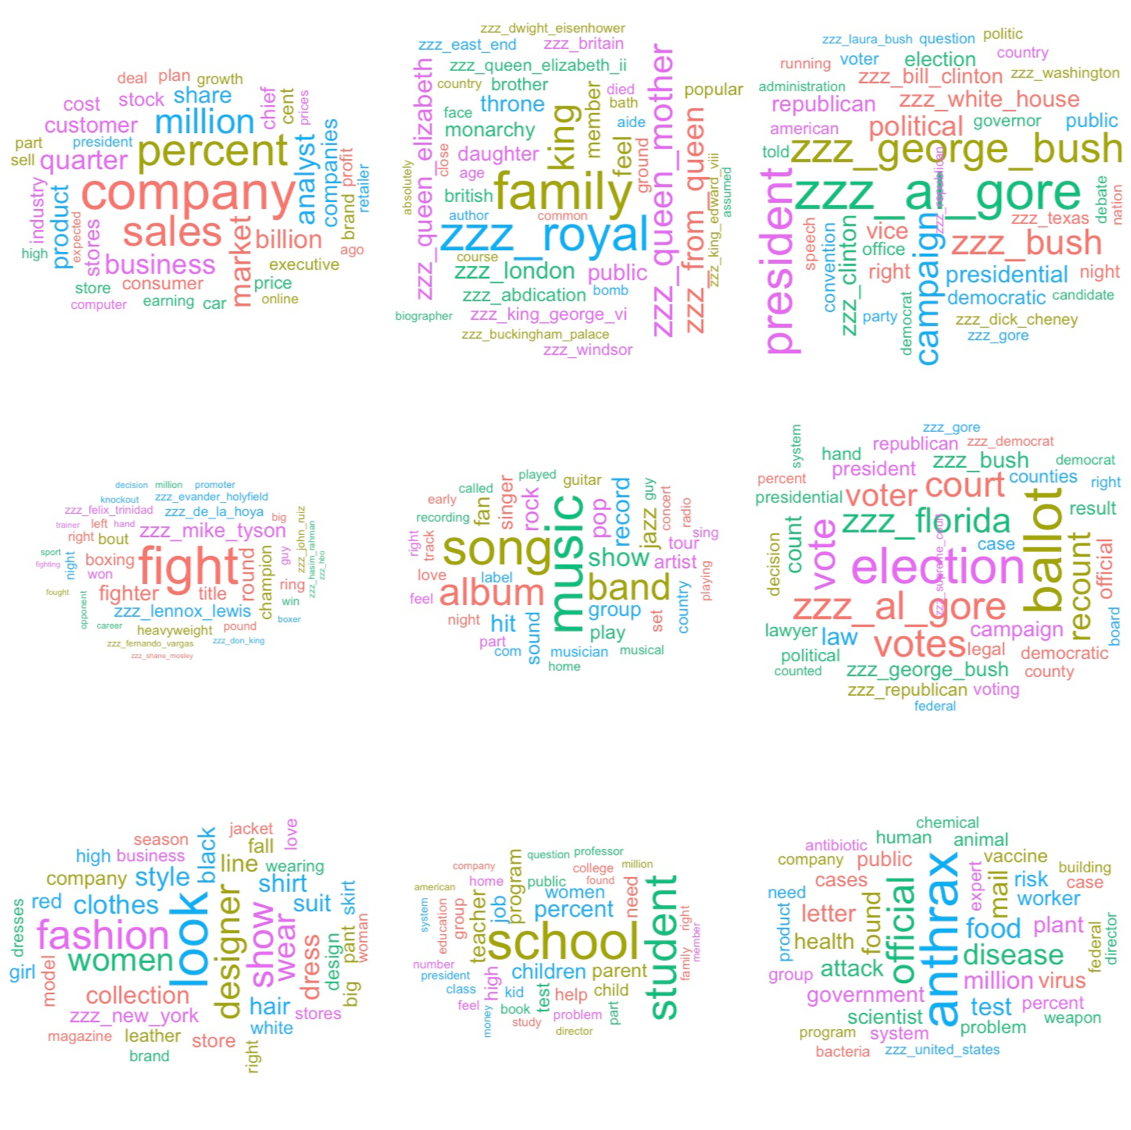
\includegraphics[width=0.5\textwidth]{img/clouds.png}
\caption{Word Clouds from NYTimes Clusters}
\label{fig:clouds}
\end{figure}


\section{Conclusion}

We successfully implemented sequential and parallel versions of Collapsed Gibbs Sampler, Direct Gibbs Sampler and Split-Merge Sampler in Julia, in a fast and accurate manner. The bodies of the algorithms are implemented in such a way that they bear the simplicity of the pseudocodes presented here in the sections above. This is inline with our design goal of providing an easy-to-understand implementation. Therefore, we are not investigating the actual implementations of the algorithms in detail here, as one can always refer to the code repository and functional documentation for detailed information.

The results shows that DPMM.jl outperforms other existing packages in single core and multi core performances for both Gaussian and Multinomial data. It doesn't yet provide multi-machine parallelism which we leave as a future work. 


\bibliography{cite}

\end{document}
